\documentclass[hidelinks, 12pt]{article}
\usepackage{fontspec}
\usepackage{xunicode}
\usepackage[french]{babel}

\usepackage{csquotes}
\usepackage[style=verbose-ibid,backend=bibtex]{biblatex}

\usepackage{hyperref}
\usepackage{enumitem}
\usepackage{setspace}
\usepackage{lscape}
\usepackage{graphicx}
\usepackage{float}

\usepackage{soul}
\usepackage{color}
\usepackage[dvipsnames]{xcolor}
\usepackage{listings}

\newcommand{\code}[1]{\colorbox{LightGray}{\texttt{#1}}}

\definecolor{LightGray}{rgb}{0.97,0.97,0.97}
\definecolor{red}{RGB}{255,0,0}
\definecolor{brown}{RGB}{139,69,19}
\definecolor{green}{RGB}{0,128,0}
\definecolor{blue}{RGB}{0,0,255}

\lstdefinelanguage{SPARQL}{
	basicstyle=\small\ttfamily,
	backgroundcolor=\color{LightGray},
	%	
	tabsize=1,
	showstringspaces=false,
	columns=fullflexible,
	breaklines=true,
	breakatwhitespace=true,
	%
	aboveskip=1em,
	belowskip=1em,
	xleftmargin=.5em,
	xrightmargin=.5em,
	framexleftmargin=.5em,
	framextopmargin=.5em,
	framexbottommargin=.5em,
	framexrightmargin=.5em,
	%
	morekeywords=[1]{paysLabel,population,date,cio,pays,populationStatement},
	keywordstyle=[1]\color{green},
	%
	morekeywords=[2]{wd,Q6256,wdt,P31,p,P1082,ps,pq,P585,wikibase,P984,label,bd,serviceParam,language},
	keywordstyle=[2]\color{MidnightBlue},
	%
	morekeywords=[3]{SELECT,ORDER,BY,WHERE,FILTER,YEAR,NOW,SERVICE},
	keywordstyle=[3]\color{red},
	%
	morestring=[b][\color{brown}]",
	otherkeywords={?},
}

\lstdefinelanguage{python}{
	basicstyle=\small\ttfamily,
	backgroundcolor=\color{LightGray},
	%	
	tabsize=1,
	showstringspaces=false,
	columns=fullflexible,
	breaklines=true,
	breakatwhitespace=true,
	%
	aboveskip=1em,
	belowskip=1em,
	xleftmargin=.5em,
	xrightmargin=.5em,
	framexleftmargin=.5em,
	framextopmargin=.5em,
	framexbottommargin=.5em,
	framexrightmargin=.5em,
	%
	morekeywords=[1]{import,as,for,in,True},
	keywordstyle=[1]\color{Fuchsia},
	%
	morekeywords=[2]{FMI\_prepared2,FMI\_prepared2\_df,colonnes\_a\_traiter,colonne,condition,keep,subset,FMI\_Python},
	keywordstyle=[2]\color{MidnightBlue},
	%
	morekeywords=[3]{dataiku,pandas,pd},
	keywordstyle=[3]\color{green},
	%
	morestring=[b][\color{brown}]",
	morestring=[b][\color{brown}]',
	otherkeywords={?},
}


\bibliography{Journal-de-bord-bibliographie}

\title{Projet Jeux Olympiques - Journal de bord}
\date{Janvier 2024}
\author{T. Burnel, N. Grim, M. Griveau, M. Mechentel}

\begin{document}

\setstretch{1.5}
\maketitle





















\section{Introduction}

Nous sommes une équipe de datajournalistes chargée, à l'approche des Jeux Olympiques de Paris, d'étudier l'existence ou non de liens entre le succès d'un pays aux Jeux Olympiques et sa richesse. Notre rôle sera de comparer le nombre de médailles remportées par pays et par sport à six éditions des Jeux (1996, 2000, 2004, 2008, 2012, 2016) pour cerner la présence ou l'absence d'une logique économique dans la réussite des pays.

Notre hypothèse de départ est la suivante : les pays développés gagnent significativement plus de médailles en raison de leur niveau d'investissement dans le sport. À l’aune de l’examen et du traitement des données, nous avons pour ambition de déterminer si la politique d’investissement dans les infrastructures sportives de ces pays influe -- tant positivement que négativement -- sur leurs résultats aux différentes épreuves des Jeux Olympiques.

Notre travail consistera, dans un deuxième temps, en une analyse comparative de la politique d'investissement du Royaume-Uni et de la France. Plusieurs points de convergence distinguent ces deux pays : leur nombre d'habitants, leur économie et leur qualité de pays organisateur des Jeux.
	
Le résultat du traitement des données constituera une base à la réalisation de datavisualisations et d'une application web pouvant servir de base à l'écriture d'articles journalistiques.





















\section{Jeux de données}

\subsection{Jeux du premier \emph{flow}}

En amont de la constitution de notre premier \emph{flow}, nos jeux étaient au nombre de deux. Ils présentent les informations suivantes :
\begin{itemize}
	\item Nombre de médailles remportées par sportif et par pays sur 120 ans\autocite{kaggle} ;
	\item Le PIB des pays et leur investissement dans le domaine du sport\autocite{fmi} ;
\end{itemize}

Un troisième jeu a dû faire son entrée au cours du traitement pour pallier la maigre qualité des données fournies par le Fonds Monétaire International (\emph{confer infra}. p. \pageref{banquemondiale}), singulièrement à propos du PIB. Ce jeu provient du site de la Banque mondiale\autocite{worldbank}.

Enfin, un problème récurrent nous a poussé à la recherche d'un quatrième jeu. Lorsque Dataiku identifie des données comme \emph{country}, nous pensions pouvoir en extraire les coordonnées et les croiser avec d'autres jeux. L'extension \emph{reverse geocoding plugin} aurait dû nous le permettre -- sans succès. Nos suppositions portent sur notre version gratuite de Dataiku et de son nombre réduit de fonctionnalités. Nous avons rapidement trouvé un jeu, mis à disposition sur GitHub\autocite{github}, rassemblant les données nécessaires.

Une opération obligatoire dans notre traitement consiste à enrichir ces jeux avec le résultat d'une requête SPARQL, saisie sur le service de Wikidata. Ce premier \emph{flow} a donc a sa base un ensemble de cinq jeux.





\subsubsection{Jeu de Kaggle}

Le jeu présente 15 colonnes pour 271117 lignes. Il contient des colonnes informatives sur les athlètes (ID ; Name ; Sex ; Age ; Height ; Weight), sur leur pays (Team ; NOC) et sur les Jeux : l'édition, l'année, la saison, la ville d'accueil, le sport et l'épreuve (Games ; Year ; Season ; City ; Sport ; Event) ainsi que sur les médailles remportées (Medal).

La propreté du jeu est notable, seules certaines données sur la taille et le poids des athlètes sont manquantes. La gravité de ces absences est toute relative dans la mesure où ne comptons pas conserver ces données. Un problème plus préoccupant concerne le nom de certains États, aujourd'hui obsolète (Allemagne de l'Est, Yougoslavie, Tchécoslovaquie, Union Soviétique, etc.).





\subsubsection{Jeu du FMI}

Le jeu présente 41 colonnes pour 7715 lignes. Il est issu d'un requêtage depuis le site du FMI pour récupérer les données avec lesquelles nous souhaitions travailler. Le potentiel de croisement est limité car un certain nombre de colonnes fournit des codes et des désignations propres au FMI (Country Code ; COFOG Function Name ; COFOG function Code ; Sector Name ; Unit Name ; Unit Code ; Attribute).

29 colonnes correspondent aux années couvertes par le FMI : de 1993 à 2022. Notre intérêt repose singulièrement sur les colonnes de 1996 à 2016 en plus des colonnes \emph{Country Name}, \emph{COFOG Function Name} laquelle correspond aux investissement dans les infrastructures sportives et \emph{Unit Name}, c'est-à-dire l'échelle de mesure, soit en PIB soit en monnaie courante.

Ce jeu est de loin le moins bien structuré et le plus fautif. En guise d'exemple, les trois dernières colonnes (Indicator Code ; Global DSD Time Series Code ; col\_41) sont d'une opacité confondante et témoignent du majeur problème du jeu : énormément de données sont vides, nulles ou incompréhensibles (\enquote{GERS\_G14\_GDP\_PT} pour la colonne) \emph{Indicator Code}, \enquote{A|GB|S1311|W0|S1|G2M|\_Z|\_Z|GF0801|XDC|\_T|\_X} pour la colonne \emph{Global DSD Time Series Code}). En somme, ce jeu représente un véritable enjeu de nettoyage et de croisement des données.





\subsubsection{Jeu de la Banque mondiale}

Le jeu présente 67 colonnes pour 541 lignes -- en réalité 271 : il faut soustraire une ligne (l'entête) et diviser le nombre de lignes par deux car chaque ligne pleine est séparée de la suivante par une ligne vide. L'essentiel des colonnes correspondent à une période chronologique : de 1960 à 2022. Les autres fournissent des informations à propos des pays (Country Name ; Country Code) et leur PIB (Indicator Name ; Indicator Code) -- notons que tout est indiqué en dollar courant, il n'y a pas de monnaie domestique.

Les premières décennies souffrent d'un cruel manque de données mais plus nous avançons dans le temps, plus le jeu est complet. 





\subsubsection{Jeu de GitHub}

Le jeu présente 6 colonnes pour 245 lignes. Une colonne \emph{Country} pour le nom des pays, les colonnes \emph{Alpha-2 code}, \emph{Alpha-3 code}, \emph{Numeric code} correspondent à des codes prévus par la norme ISO 3166-1 et \emph{Latitude (average)} et \emph{Longitude (average)} pour les coordonnées géographiques. Le niveau de propreté est remarquable, sans donnée manquante ou fautive.





\subsubsection{Enrichissement Wikidata sur la population}

Dans l'optique d'enrichir nos données \emph{via} Wikidata, nous avons mis au point une requête SPARQL à même de renvoyer le nombre d'habitants de l'ensemble des pays du monde sur une période de trente ans (1993 - 2003) :
		
\begin{lstlisting}[language=SPARQL]
	SELECT ?paysLabel ?population ?date ?cio
	WHERE 
	{
		?pays wdt:P31 wd:Q6256.
		?pays wdt:P984 ?cio.
		?pays p:P1082 ?populationStatement.
		?populationStatement ps:P1082 ?population. 
		?populationStatement pq:P585 ?date.
		FILTER(YEAR(?date) >= (YEAR(NOW()) - 30)).
		SERVICE wikibase:label { bd:serviceParam wikibase:language "[AUTO_LANGUAGE],fr". }
	}
	ORDER BY ?paysLabel ?date
\end{lstlisting}

Être en mesure de requêter l'intégralité des pays a été la première étape de la construction de notre requête. Le premier triplet permet de spécifier la nature -- notée \code{wdt:P31} -- de notre variable inconnue \code{?pays} en la faisant correspondre à l'objet \code{country} -- noté \code{wd:Q6256} :
		
\begin{lstlisting}[language=SPARQL]
	?pays wdt:P31 wd:Q6256.
\end{lstlisting}

Le deuxième triplet constitue un ajout tardif, destiné à faciliter les jointures avec les autres jeux de données. Comme nous travaillons sur les Jeux Olympiques, les pays peuvent être non seulement identifiés par les codes basés sur la norme ISO 3166 mais aussi par les codes du CIO (Comité International Olympique). Nous avons donc récupéré cette donnée grâce à la propriété Wikidata correspondante -- notée \code{wdt:P984} :

\begin{lstlisting}[language=SPARQL]
	?pays wdt:P984 ?cio.
\end{lstlisting}

La deuxième partie de notre requête doit renvoyer le nombre d'habitants par pays en prenant en compte une dimension chronologique. La complexité de cette demande requiert un parcours de graphique en quatre temps.

Pour ce faire, nous avons consulté la liste de préfixes\autocite{wikiprefixes} de Wikidata afin de créer une nouvelle variable, \code{?populationStatement}. Le troisième triplet a recours à la classe \code{population} -- notée \code{p:P1082} -- et signifie que la variable \code{?populationStatement} a pour valeur la population des pays :

\begin{lstlisting}[language=SPARQL]
	?pays p:P1082 ?populationStatement.
\end{lstlisting}

L'obtention du nombre d'habitants a nécessité le recours au préfixe \code{ps}, lequel permet de récupérer la valeur de la propriété relative à la population :
		
\begin{lstlisting}[language=SPARQL]
	?populationStatement ps:P1082 ?population.
\end{lstlisting}

Enfin, nous avons rédigé le dernier triplet sur la base du préfixe \code{pq} pour attribuer la valeur chronologique à la variable \code{?date}. Un filtre y a été appliqué pour exprimer les limites extrêmes de notre période, soit \code{NOW} pour 2023 et \code{-30} pour 1993 :
	
\begin{lstlisting}[language=SPARQL]
	?populationStatement pq:P585 ?date.
	FILTER(YEAR(?date) >= (YEAR(NOW()) - 30)).
\end{lstlisting}

La première et dernière ligne permettent de cadrer l'affichage des résultats. Lorsque la requête s'exécute, Wikidata renvoie le nom de chaque pays (\code{?paysLabel}) par ordre alphabétique, le nombre d'habitants (\code{?population}) et l'année correspondante (\code{?date}) par ordre croissant :

\begin{lstlisting}[language=SPARQL]
	SELECT ?paysLabel ?population ?date
	ORDER BY ?paysLabel ?date
\end{lstlisting}

Nous nous sommes heurtés à plusieurs obstacles avant de rendre la requête fonctionnelle. Il nous a fallu un certain temps avant de comprendre la nécessité d'un parcours de graphique en quatre temps et du recours à une variable telle que \code{?paysStatement}. À cet égard, la documentation sur l'utilisation des propriétés \code{population}\autocite{wikipop} et \code{date}\autocite{wikidate} a été d'un grand secours. 

Nous avons également pris en exemple la requête \emph{Population in Europe after 1960}\autocite{wiki1960}. La consulter a été l'occasion d'une meilleure compréhension des propriétés Wikidata ainsi qu'une porte ouverte à la lecture de la documentation et à l'appréhension des requêtes en deux temps (collecte des propriétés d'une classe puis requêtage en fonction de notre besoin).





















\subsection{Jeux du second \emph{flow}}

Notre deuxième \emph{flow} repose sur la comparaison entre les investissements de la France et du Royaume-Uni, en l'occurrence à l'endroit des infrastructures de natation. En amont du traitement, nos jeux de données étaient au nombre de trois et présentent les informations suivantes :

\begin{itemize}
	\item Investissements dans les infrastructures sportives en France\autocite{ministere} ;
	\item Investissements dans les infrastructures sportives au Royaume-Uni\autocite{ru}.
\end{itemize}


\subsubsection{Jeu du ministère des sports et des jeux olympiques et paralympiques}

Le jeu présente 114 colonnes pour 143192 lignes. Par souci de concision, nous ne nous attarderons que sur les données qui seront conservées. Les colonnes concernées sont \emph{Type d'équipement sportif} et \emph{Commune Ancienne}, laquelle renseigne les codes postaux.

Sur l'ensemble du jeu, les données sont grossièrement saisies. Les \emph{Type d'équipement sportif} sont par exemple au nombre de 354 sans harmonisation commune dans la nomenclature avec présence de données aberrantes (citons \enquote{3 2}, \enquote{PETIT MORNAS} ou encore \enquote{Puy}). Nous nous appuierons sur la colonne \emph{Commune Ancienne} non pas sur la colonne \emph{Région Nom} car les données sont également mal saisies et aberrantes (\enquote{CC du Pays Châtillonnais}, \enquote{4.84405}, etc.).

\subsubsection{Jeu de Sport England}

À l'endroit du Royaume-Uni : deux jeux nous intéressent. Le premier, nommé \emph{Geographics} présente -- sur 25 colonnes et 118655 lignes -- des données géographiques à propos d'infrastructures sportives. Chaque infrastructure possède son ID (\emph{FacilityID}) et est rattachée à une région. Les autres colonnes fournissent des informations à propos des régions, selon un principe de colonne jumelles avec d'une part les ID, d'autre part les noms (Parliamentary Constituency ID ; Ward, Local Authority, Country, Active Partnership, Region). Deux colonnes concernent les coordonnées (\emph{Latitude} ; \emph{Longitude}).

Sur la propreté des données, certaines colonnes sont entièrement vides (\emph{Metro Name} ; \emph{Core City Name} ; \emph{LDP Code} ; \emph{LDP Name}) mais nous ne comptons pas les conserver au cours du traitement. Nonobstant, les données des coordonnées correspondent aux infrastructures, non pas aux régions. Cela pourra avoir des conséquences sur les visualisations dans la mesure où la myriade de points ne saura faire ressortir les contours des régions. 

Le second jeu se nomme \emph{SwimmingPool} et fournit des données sur la répartition des équipements de natation au Royaume-Uni. L'essentiel des colonnes donne des détails techniques sur les infrastructures (\emph{Length} ; \emph{Maximum Depth} ; \emph{Movable Floor} ; \emph{Seating}, etc.).

L'intégralité des données sont des entiers. Les entrées vides ou équivalentes à zéro sont derechef légion. Cependant, seule la colonne \emph{FacilityID} nous est nécessaire afin de réaliser des jointures avec le jeu \emph{Geographics}. 




















\section{Traitement des données}
	
\subsection{Objectif du traitement}
		
\subsection{Chaîne de traitement}

\subsubsection{Semaine du 1\textsuperscript{er} janvier 2024}
		
Nous avons constaté que le jeu de données du FMI est trop avare en données fiables (données manquantes, valeurs aberrantes\footnote{Donner des exemples.}) à propos des investissements en pourcentage du PIB dans le domaine du sport. Nous avons donc fait le choix d'utiliser les valeurs absolues\footnote{?} que nous croiserons avec le PIB par habitant de chaque pays.
		
Pour ce faire, nous avions de prime abord songé à rédiger une autre requête SPARQL. Nonobstant, le résultat ne concernait que les années 2021 et 2022 -- les années précédentes sont vraisemblablement absentes de Wikidata.
		
\label{banquemondiale}Nous avons donc dû trouver un jeu de données contenant le PIB par habitant. Parmi les données sources de Wikidata se trouvait un jeu hébergé sur le site de la Banque mondiale. Les données correspondent à une profondeur temporelle suffisante pour le cadre de notre projet. Cela nous a permis de résoudre le problème de mauvaise qualité du jeu du FMI.



\begin{lstlisting}[language=python]
import dataiku
import pandas as pd
from dataiku import pandasutils as pdu

FMI_prepared2 = dataiku.Dataset("FMI_prepared2")
FMI_prepared2_df = FMI_prepared2.get_dataframe()

colonnes_a_traiter = ['1996 - FMI', '2000 - FMI', '2004 - FMI', '2008 - FMI', '2012 - FMI', '2016 - FMI']

for colonne in colonnes_a_traiter:
	condition = FMI_prepared2_df[colonne] > 0.1
	FMI_prepared2_df.loc[condition, colonne] /= 10

FMI_prepared2_df.drop_duplicates(subset=['Pays'], keep='first', inplace=True)

FMI_Python = dataiku.Dataset("FMI_Python")
FMI_Python.write_with_schema(FMI_prepared2_df)
\end{lstlisting}




\subsubsection{Semaine du 22 janvier 2024}

Mauvaise surprise : alors que nous voulions produire un autre flow afin de remplir la seconde partie de notre objectif et produire des datavisualisations comparant la France et le Royaume-Uni, un bogue manifestement causé par une installation relative à Javascript perturbe l'affichage sur Dataiku. Probablement : problèmes de compatibilité.

\begin{center}
	\begin{figure}[H]
		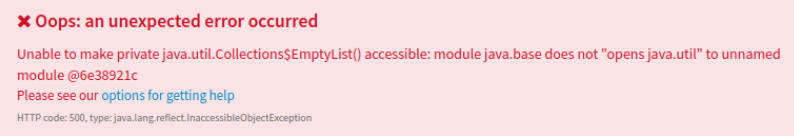
\includegraphics[scale=0.5]{bogue.png}
	\end{figure}
\end{center}

ll est probable que cette erreur soit apparue après l’installation d’une version de JDK supérieure à celle prise en charge par Dataiku. Il aurait ainsi fallu rétrograder notre version de JDK, mais nous craignons que cette manipulation entraîne des difficultés dans d’autres projets que nous menons. Nous ne pouvons dès lors nous appuyer que sur un seul ordinateur, qui possède une version inférieure de JDK, ce qui a causé d’importants soucis organisationnels à la fin du mois de janvier.


\section{Visualisation des données}

\subsection{Présentation des visualisations}

\subsection{Analyse}

Qu'apprend-on en regardant les visualisations ? Quels sont les biais ?
\newpage


\section{Sitographie}
\printbibliography[heading=none]
\newpage

\tableofcontents

\end{document}